\subsection{Check-Round Layouts}
\label{sub:ancilla_layouts}

% Sec. 2.4 (track hw). Former Sec. 3.2.3 (method - LRB-D.tex, lines 172-210 of the 438f6f16 mirror). The syndrome-extraction circuits, the relay walk-through and the gate-moment table (tab:conv_round) are in Appendix B.
% Gate and moment counts of both rounds: paper-rework/scratch/writer-conv/budget.py (budget.out) and jpw-review/hw/checks/check_fault_budgets.py (.out). Single-fault enumeration of both simulated rounds: jpw-review/hw/checks/check_single_faults.py (.out)
Which check round a device can run depends on its connectivity. We therefore compare two layouts of the code on the conventional surface-code grid (\autoref{fig:ancilla_layouts}). The grid has one data qutrit at the center of a square, the other four at its corners, and four ancilla sites, each next to the center and to two adjacent corners. Both layouts use nine qutrits. In the check rounds of both, each ancilla couples only to its neighboring data qutrits, and no two ancillas are coupled. The layouts differ in which data qutrit sits at the center.

% ============================================================
% fig - ancilla layouts.tex
% Terminal postselection, one-ancilla and two-ancilla (conventional-site)
% check layouts on the conventional surface-code grid. The drawing is a
% standalone TikZ figure (paper-rework/layout-figure/ancilla-layouts.tex),
% compiled to figures/ancilla-layouts.pdf; the caption body lives here.
% Caption shortened by track hw (2026-11-13): the line styles are explained by
% the legend inside the figure, and the relay walk-through is in Appendix B.
% ============================================================
\begin{figure}[!tb]
  \centering
  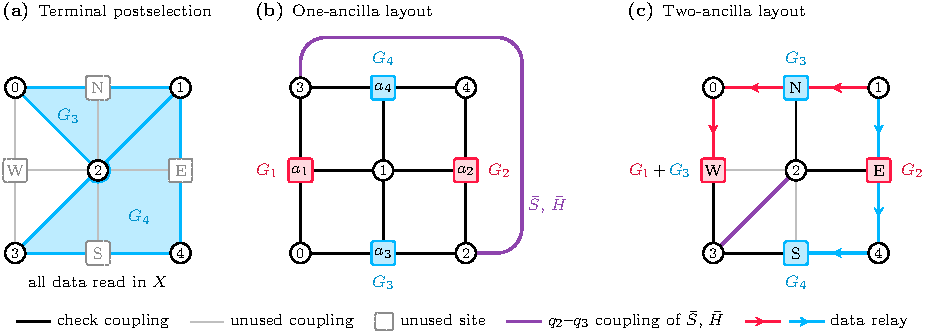
\includegraphics{figures/ancilla-layouts.pdf}% drawn at final size
  \caption{Stabilizer measurements of the $[[5,1,2]]_3$ code on the conventional surface-code grid of data qutrits (circles, labeled by their index) and ancilla sites (squares). Red marks the $Z$-type stabilizers $G_1$, $G_2$ and blue the $X$-type $G_3$, $G_4$. The label beside a site is what the site reads out once per check round, modulo three and up to a sign.
(a)~Terminal postselection uses no ancillas: the final $X$-basis readout of all data qutrits gives $G_3$ and $G_4$ (shaded).
(b)~One-ancilla layout, with $q_1$ at the center. Ancilla $a_j$ neighbors the three data qutrits of $G_j$, and the two-qutrit gates of $\bar H$ and $\bar S$ need a long-range coupling between $q_2$ and $q_3$.
(c)~Two-ancilla layout, with $q_2$ at the center and the sites N, W, E and S. $q_2$ and $q_3$ are diagonal neighbors, and $G_1$ and $G_4$ use two sites each. Arrows trace the data relay: N lends its part of $G_1$ to $q_0$, where W collects it, so that W reads $G_1$ shifted by the value of $G_3$ that N holds, and E lends its part of $G_4$ to $q_4$, where S collects it.}
  \label{fig:ancilla_layouts}
\end{figure}


\paragraph{One-ancilla layout.} With $q_1$ at the center (\autoref{fig:ancilla_layouts}(b)), every stabilizer acts on the center and two adjacent corners, so each $G_j$ has a site next to all three of its data qutrits and is measured there by its own ancilla $a_j$. The extraction circuits are the standard ones, with SUM gates and their inverses in place of CNOT gates (\autoref{app:rounds}). We count the length of a round in moments, sets of operations on disjoint qutrits that run in parallel. The round takes nine moments: one for the resets, seven for its 12 two-qutrit and four one-qutrit gates, and one for the readouts. In this layout $q_2$ and $q_3$ sit at opposite corners, so the two-qutrit gates of $\bar H$ and $\bar S$ need a long-range coupling.

\paragraph{Two-ancilla layout.} With $q_2$ at the center (\autoref{fig:ancilla_layouts}(c)), as on the patch of \autoref{fig: 5-qutrit-code}, the logical gates couple diagonal neighbors, but two stabilizers lose their site. $G_2$ and $G_3$ still have a site next to their three data qutrits. $G_1$ and $G_4$ each contain the opposite corners $q_1$ and $q_3$ and have no such site. We call these two generators, which do not contain $q_2$, the boundary stabilizers. Each of them is measured with two sites. Reading the two parts of a boundary stabilizer on separate sites would not measure it (\autoref{app:rounds}). Instead, the first site collects its part and lends it to a data qutrit next to both sites, the second site collects it there and collects the rest of the stabilizer, and the first site takes its part back, all before any site is read. We call this scheme a data relay. Every site is read once per round, and the four readouts are zero exactly when the four syndromes are trivial. As in the one-ancilla round, a single Pauli fault in an otherwise noiseless round never leads to a logical error that this round and the next both miss (\autoref{app:rounds}). The round takes 13 moments, 11 of them for its 18 two-qutrit and six one-qutrit gates.

In the simulations the two layouts differ only in the check round. Both use the same code, logical gates, encoding and logical readout, and the $q_2$--$q_3$ gates receive the same noise as any other two-qutrit gate, wherever $q_2$ and $q_3$ sit (\autoref{sub:noise_models}). The comparison therefore leaves out the cost of the long-range coupling. What remains is the data relay, which adds six two-qutrit gates, two one-qutrit gates and four gate moments to the round.
